\documentclass[a4paper, 11pt]{article}
\usepackage[polish]{babel}
\usepackage[MeX]{polski}
\usepackage[utf8]{inputenc}
\usepackage[T1]{fontenc}
%\usepackage{times}
\usepackage{graphicx,wrapfig}
\usepackage{pdfpages}
%\usepackage{anysize}
%\usepackage{tikz}
%\usetikzlibrary{calc,through,backgrounds,positioning}
\usepackage{anysize}
\usepackage{float}
%\usepackage{stmaryrd}
%\usepackage{amssymb}
%\usepackage{amsthm}
%\marginsize{3cm}{3cm}{3cm}{3cm}
%\usepackage{amsmath}
%\usepackage{color}
%\usepackage{listings}
%\usepackage{enumerate}


\begin{document}
	% \noindent -  w tym akapicie nie bedzie wciecia
	% \ indent - to jest aut., ale powoduje ze jest wciecie
	% \begin{flushleft}, flushright, center - wyrownianie akapitu
	% \textbf{pogrubiany tekst}
	% \textit{kursywa} 
	% 					STRONY 
	%  http://www.codecogs.com/latex/eqneditor.php 
	%  http://www.matematyka.pl/latex.htm
	% 
	\begin{titlepage}
	
	
		
		\newcommand{\HRule}{\rule{\linewidth}{0.5mm}} % Defines a new command for the horizontal lines, change thickness here
		
		\center % Center everything on the page
		
		%----------------------------------------------------------------------------------------
		%	HEADING SECTIONS
		%----------------------------------------------------------------------------------------
		
		\textsc{\LARGE Akademia Górniczo-Hutnicza im. Stanisława Staszica w Krakowie}\\[1.5cm] % Name of your university/college
		\textsc{\Large Inżynieria Oprogramowania}\\[1.5cm]
		%\textsc{\Large Krak�w}\\[0.5cm] % Major heading such as course name
		%\textsc{\large }\\[0.5cm] % Minor heading such as course title
		
		%----------------------------------------------------------------------------------------
		%	TITLE SECTION
		%----------------------------------------------------------------------------------------
		
		\HRule \\[0.4cm]
		{\fontsize{38}{50}\selectfont System Zarządzania Apteką}
	%	{ \Huge \bfseries} Symulator po�aru lasu\\[0.3cm] % Title of your document
		\HRule \\[5.5cm]
		
		%----------------------------------------------------------------------------------------
		%	AUTHOR SECTION
		%----------------------------------------------------------------------------------------
		
		% If you don't want a supervisor, uncomment the two lines below and remove the section above

\begin{minipage}{0.4\textwidth}
\begin{flushleft} \large 
\emph{Autorzy:}\\
Marcin \textsc{Jędrzejczyk}\\ % Your name
Paweł \textsc{Ogorzały} \\

\end{flushleft}
\end{minipage}
~
\begin{minipage}{0.4\textwidth}
\begin{flushright} \large
\emph{Prowadzący:}\\
 Dr inż. Radosław \textsc{Klimek}  % Supervisor's Name
\end{flushright}
\end{minipage} \\[5cm]

		
		%----------------------------------------------------------------------------------------
		%	DATE SECTION
		%----------------------------------------------------------------------------------------
		
		{\large \today}\\[3cm] % Date, change the \today to a set date if you want to be precise
		
		%----------------------------------------------------------------------------------------
		%	LOGO SECTION
		%----------------------------------------------------------------------------------------
		
		%\includegraphics{Logo}\\[1cm] % Include a department/university logo - this will require the graphicx package
		
		%----------------------------------------------------------------------------------------
		
		\vfill % Fill the rest of the page with whitespace
		
	\end{titlepage}
	
	%SPIS TRESI
	%
	%
	%
	%
	%
	%
	%
	%
	%
	
	\tableofcontents
	\vfill

	\newpage
	
	\section{Streszczenie systemu}
	\indent
	
	Nasz projekt przedstawia system zarządzania apteką. \newline
	\newline \indent 
	Apteka zapewnia obsługę klientów na miejscu.
	Klient ma możliwość zakupu leków bez recepty oraz z receptą. Płatności może dokonać za pomocą gotówki lub kartą. Klient może otrzymać fakturę bądź paragon.  \newline 
	\newline \indent
	Za obsługę klienta  odpowiada farmaceuta. W zakresie jego obowiązków leży także składanie zamówienia na lek w przypadku jeśli zauważy, że jego stan się kończy. Farmaceuta sporządza również raport z listą recept obsłużonych, którą wysyła do Narodowego Funduszu Zdrowia. \newline
	\newline \indent
	Za stan magazynu odpowiada magazynier. Tworzy on zamówienia i aktualizuje stan magazynu. \newline   
	\newline \indent
	Całość kontroluje kierownik, która ma możliwość zatrudniania oraz zwalniania pracowników. Kontroluje on także zamówienia składane przez magazyniera.	
	\section{Lista obiektów zewnętrznych}
	Obiekty zewnętrzne:
	\begin{itemize}
	\item Klient - posiada możliwość kupna leku za gotówkę lub kartą. Może on otrzymać paragon albo fakturę, a także zrezygnować z zakupu.
	\item Farmaceuta - jego zadaniem jest obsługa klienta. Ma obowiązek złożyć zamówienie na dostawę leku, jeżeli zauważy, że jest go mało na stanie lub kończy się jego termin ważności. Raz na miesiąc wysyła raport z listą numerów recept, które obsłużył do NFZ.
	\item Kierownik - ma możliwość zatrudniania pracowników. Kontroluje zamówienia składane przez magazyniera. Tylko on może dodać nowy lek do oferty apteki.
	\item Magazynier - jest osobą odpowiedzialną za bieżący stan magazynu. Ma możliwość sprawdzania magazynu, tworzenia zamówień, aktualizowania stanu magazynu.
	\item Narodowy Fundusz Zdrowia (NFZ)- do tej instytucji wysyłamy co miesiąc raport ze sprzedaży leków na receptę. 
	\end{itemize}
	\section{Lista zdarzeń}
	
	\begin{itemize}
	\item Wybór potwierdzenia wpłaty (paragon/faktura),
	\item Wybór formy płatności (gotówka/karta),
	\item Zrezygnowanie z kupna,
	\item Dokonanie płatności,
	\item Wybranie leku(recepta/bez recepty),
	\item Brak leku,
	\item Lek przeterminowany,
	\item Sporządzenie raportu,
	\item Przyjęcie dostawy leków.
	\end{itemize}
	
%	\section{Diagram kontekstowy}

	\section{Diagramy kontekstowy}
	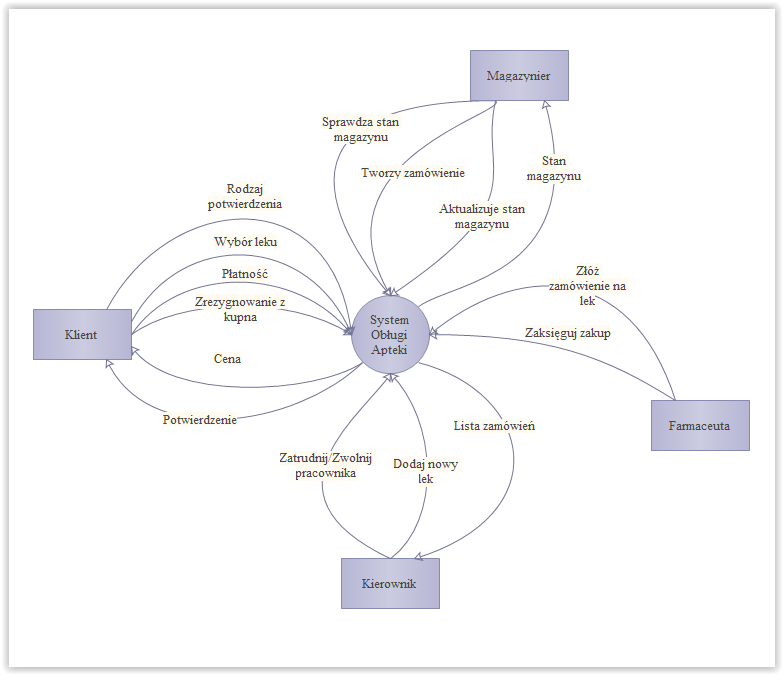
\includegraphics[scale=0.8]{zd.PNG} 
	\section{Diagram DFD-poziom 0}
		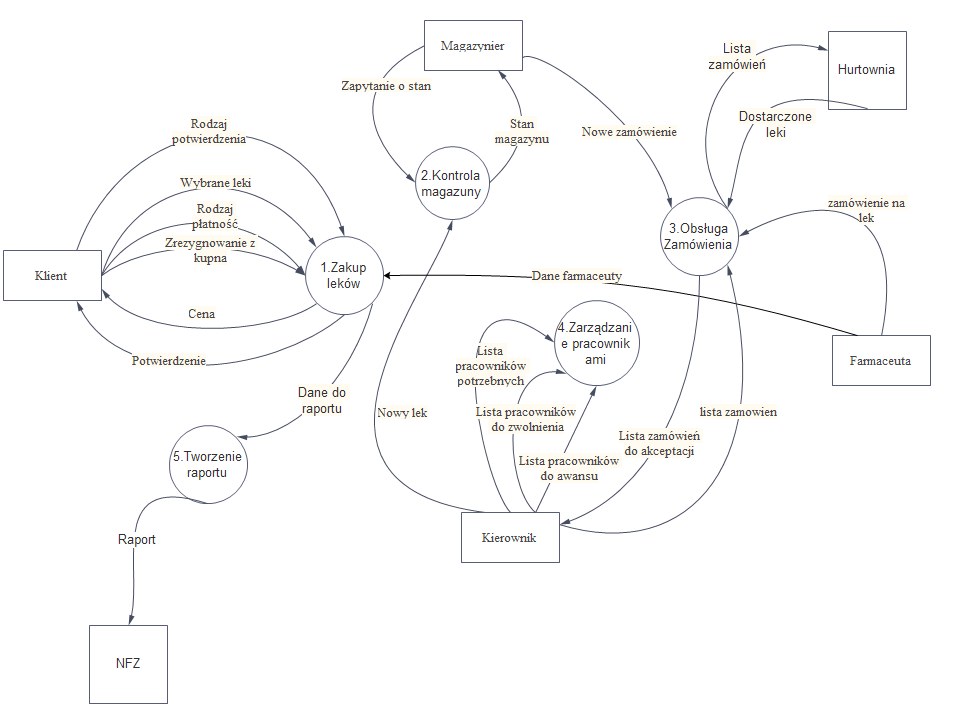
\includegraphics[scale=0.7]{dfdpoziom1.PNG} 
	
	\subsection{Diagram DFD - poziom 1 Kontrola magazynu}
		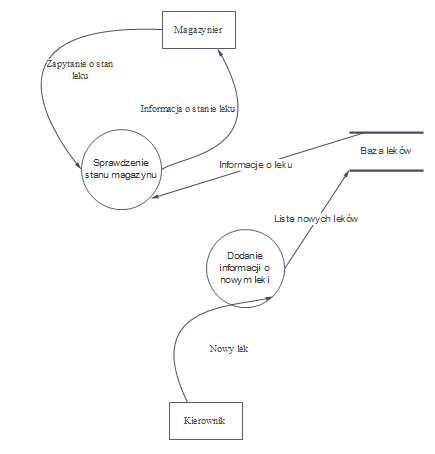
\includegraphics[scale=0.9]{kontrolaMagazynu.PNG} 
		
	\subsection{Diagram DFD - poziom 1 Zamówienia}
		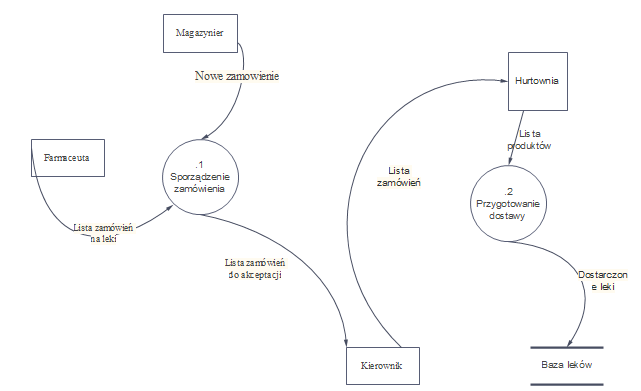
\includegraphics[scale=0.9]{zamowienia.PNG} 
		
	\subsection{Diagram DFD - poziom 1 Zarządzanie pracownikami}
		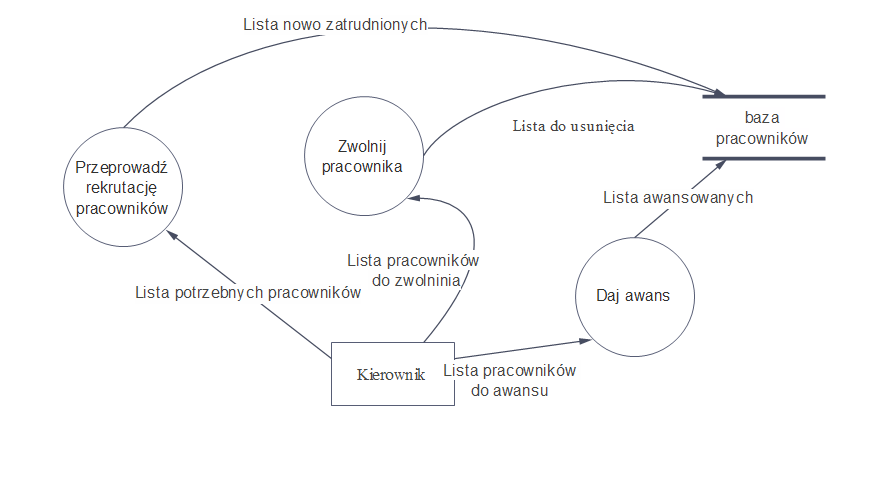
\includegraphics[scale=0.6]{zarzadzaniePracownikami.PNG} 
		
	\subsection{Diagram DFD - poziom 1 Tworzenie raportu}
		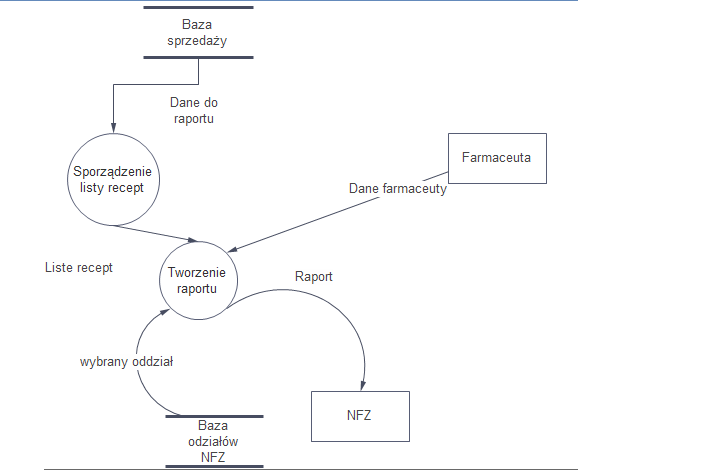
\includegraphics[scale=0.6]{tworzenieRaportu.PNG} 
		
	\subsection{Diagram DFD - poziom 1 Zakup leków}
		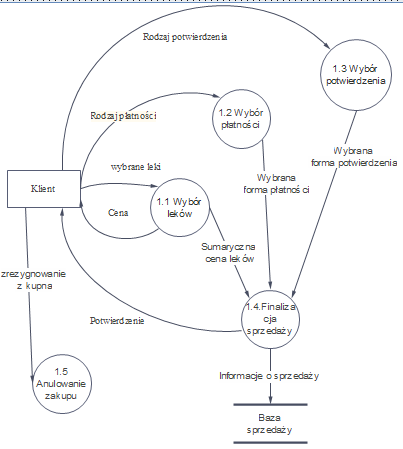
\includegraphics[scale=0.6]{zakupLekow2.PNG} 	
		\subsubsection{Poziom 2- Zakup leków- płatność gotówką}
			\begin{figure}[H]
			\centerline{\includegraphics[scale=1]{dfdp21.png}}
			\caption{Diagram STD dla raportu}
			\end{figure}
		\subsubsection{Poziom 2- Zakup leków- płatność kartą}
			\begin{figure}[H]
			\centerline{\includegraphics[scale=1]{dfdp22.png}}
			\caption{Diagram STD dla raportu}
			\end{figure}
			
	\section{Model danych diagram ERD}
	
			\begin{figure}[H]
			\centerline{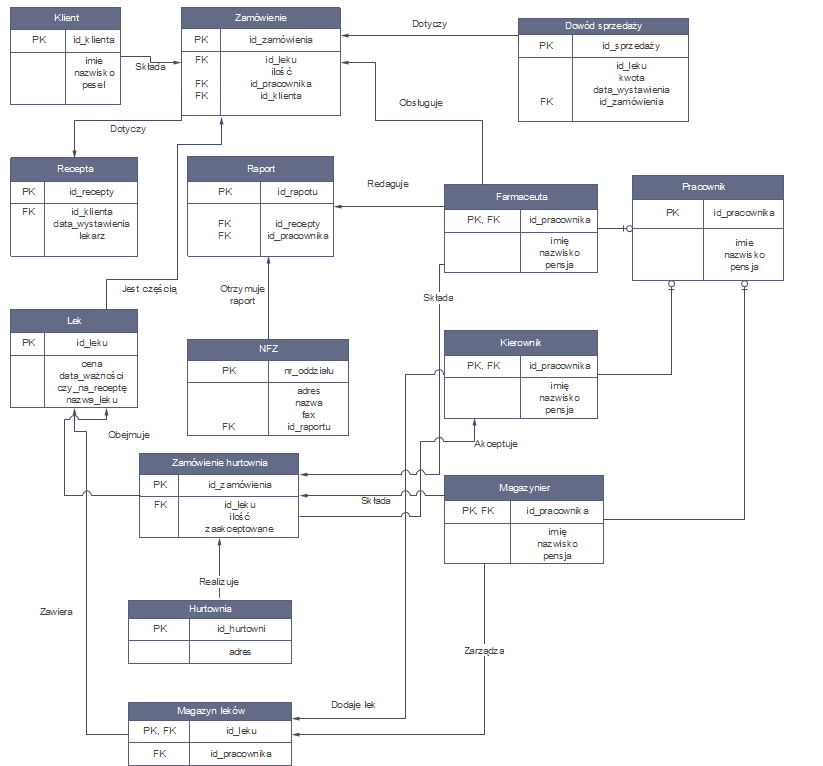
\includegraphics[scale=1]{ERD.png}}
			\caption{Diagram ERD apteki}
			\end{figure}
	\subsection{Opis atrybutów encji}
	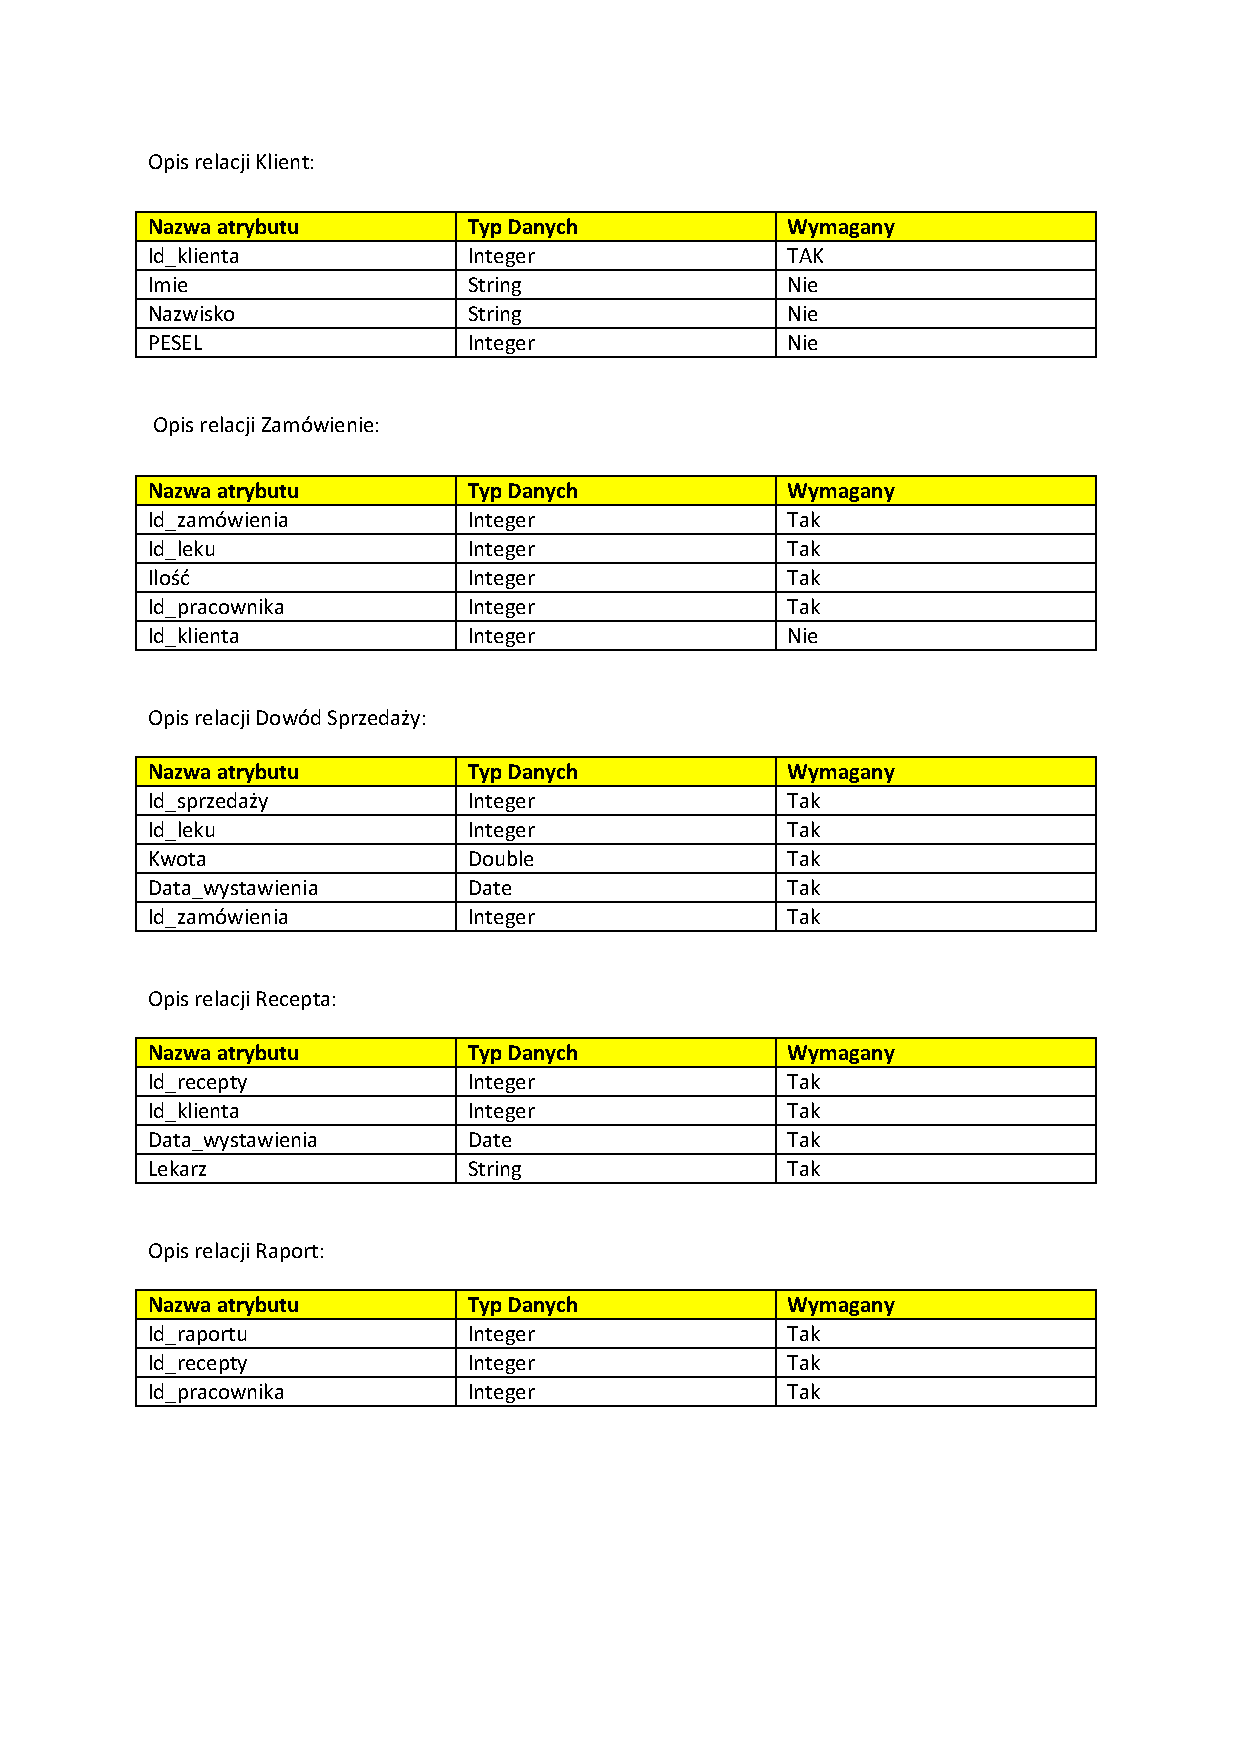
\includepdf[pages=-]{opisERD.pdf}
	
	\section{Model dynamiki systemu Diagramy STD}
	\begin{figure}[H]
\centerline{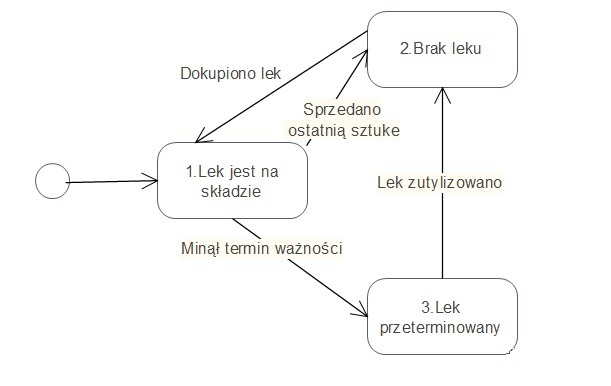
\includegraphics[scale=1]{STDlek.jpg}}
\caption{Diagram STD dla leku}
\end{figure}
	\begin{figure}[H]
\centerline{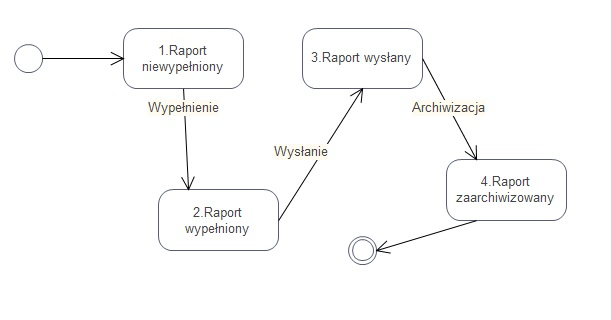
\includegraphics[scale=1]{STDraport.jpg}}
\caption{Diagram STD dla raportu}
\end{figure}

	\begin{figure}[H]
\centerline{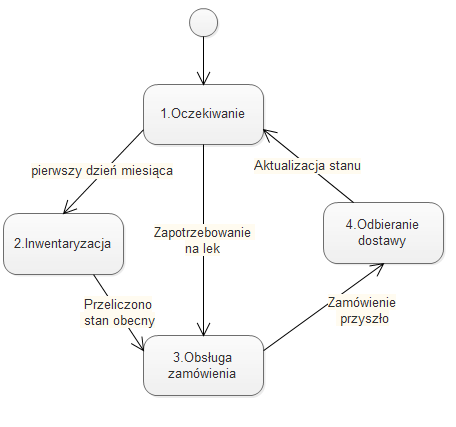
\includegraphics[scale=1]{STDmagazyn.png}}
\caption{Diagram STD dla magazynu}
\end{figure}
	\begin{figure}[H]
\centerline{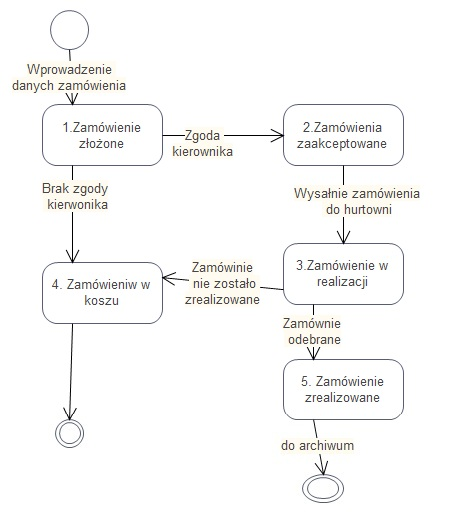
\includegraphics[scale=1]{STDzamowienie2.jpg}}
\caption{Diagram STD dla obsługi zamówienia z magazynu}
\end{figure}

	\begin{figure}[H]
\centerline{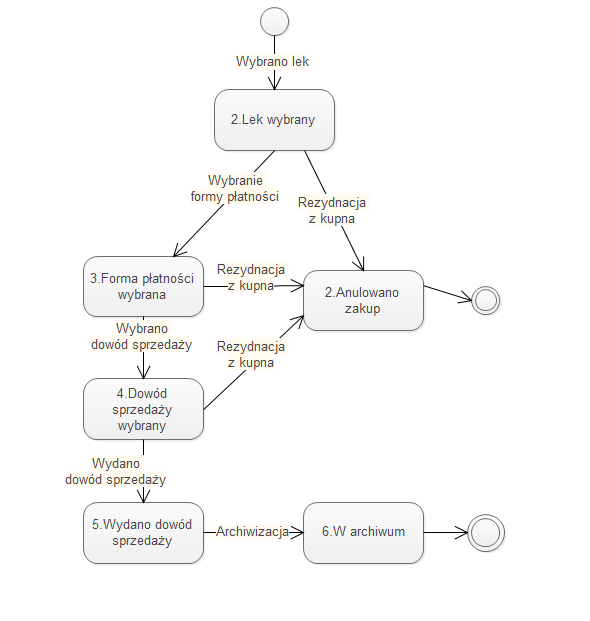
\includegraphics[scale=1]{STDzakup.png}}
\caption{Diagram STD dla zakupu leku}
\end{figure}
	\section{Słowniki danych}
	\section{Specyfikacja procesów PSPEC}
	
	
	\section{Bibliografia}
	\begin{itemize}
	\item Notatki z wykładów.
	\end{itemize}
	
\end{document}


